%!TEX root = ../../Heun_Dale_Haney_A_dynamic_approach_to_input_output_modeling.tex
%%%%%%%%%%%%%%%%%%%%% chapter.tex %%%%%%%%%%%%%%%%%%%%%%%%%%%%%%%%%
%
% sample chapter
%
% Use this file as a template for your own input.
%
%%%%%%%%%%%%%%%%%%%%%%%% Springer-Verlag %%%%%%%%%%%%%%%%%%%%%%%%%%
%\motto{Use the template \emph{chapter.tex} to style the various elements of your chapter content.}
\motto{The economy is a wholly owned subsidiary of the environment, not the reverse.
**** Need citation. ****

\hfill---\emph{Herman E. Daly}}

%%%%%%%%%%%%%%%%%%%%%%%%%%%%%%%%%%
%%%%%%%%%% Implications %%%%%%%%%%
%%%%%%%%%%%%%%%%%%%%%%%%%%%%%%%%%%
\chapter{Implications}
% Always give a unique label
\label{chap:implications}
% use \chaptermark{} to alter or adjust the chapter heading in the running head
\chaptermark{Implications}
%%%%%%%%%%%%%%%%%%%%%%%%%%%%%%%%%%
%%%%%%%%%%%%%%%%%%%%%%%%%%%%%%%%%%
%%%%%%%%%%%%%%%%%%%%%%%%%%%%%%%%%%

\abstract*{[NEED TO ADD ABSTRACT HERE]}

%% \abstract{Each chapter should be preceded by an abstract (10--15 lines long) that summarizes the content. The abstract will appear \textit{online} at \url{www.SpringerLink.com} and be available with unrestricted access. This allows unregistered users to read the abstract as a teaser for the complete chapter. As a general rule the abstracts will not appear in the printed version of your book unless it is the style of your particular book or that of the series to which your book belongs.\newline\indent
%% Please use the 'starred' version of the new Springer \texttt{abstract} command for typesetting the text of the online abstracts (cf. source file of this chapter template \texttt{abstract}) and include them with the source files of your manuscript. Use the plain \texttt{abstract} command if the abstract is also to appear in the printed version of the book.}

%% Use the template \emph{chapter.tex} together with the Springer document class SVMono (monograph-type books) or SVMult (edited books) to style the various elements of your chapter content in the Springer layout.


Several implications can be drawn from the detailed development 
of our framework for materials and energy accounting 
(in Chapters~\ref{chap:materials}--\ref{chap:intensity}).
In the sections below, we discuss 
implications for the I-O method itself,
implications for economic ``development,''
implications for recycling, reuse, and dematerialization, and
comparisons with the idea of a steady-state economy.
We begin by examining the I-O method itself 
through the lens of our framework.


%%%%%%%%%% Implications for the I-O method %%%%%%%%%%
\section{Implications for the I-O method}
\label{sec:Implications_for_IO}
%%%%%%%%%%

Extension of the Leontief\index{Leontief} 
Input-Output method\index{input-output method}
for energy analysis has allowed energy analysts to estimate 
the energy intensity\index{energy intensity}
of economic products~($\boldsymbol{\varepsilon}$). 
As discussed in Section~\ref{sec:Value_Methodology},
we do not take the ability to estimate energy intensity as a license
to declare an intrinsic ``energy theory of value.''
\index{theory of value!energy}
Rather, we belive that energy intensity~($\boldsymbol{\varepsilon}$) is an 
important and useful metric that can assess 
the energy performance of economies,
even within the prevailing subjective theory of value\index{theory of value!subjective}
that underlies modern economics.
For this reason, it is important to consider the assumptions behind
the literature's presentation of the I-O method 
for estimating the energy intensity economic output.

As we investigate, we will use the following
coordinates of analysis:
product-based vs.\ physical accounting approaches,
whether capital stock is included, and
whether society is endogenous to the economy.
(See Figure~\ref{fig:coords_of_analysis}.)
We will end with our suggestion for how best to estimate
$\boldsymbol{\varepsilon}$ within
a materials, energy, and value accounting system.

\begin{figure}[!ht]
	\centering{}
	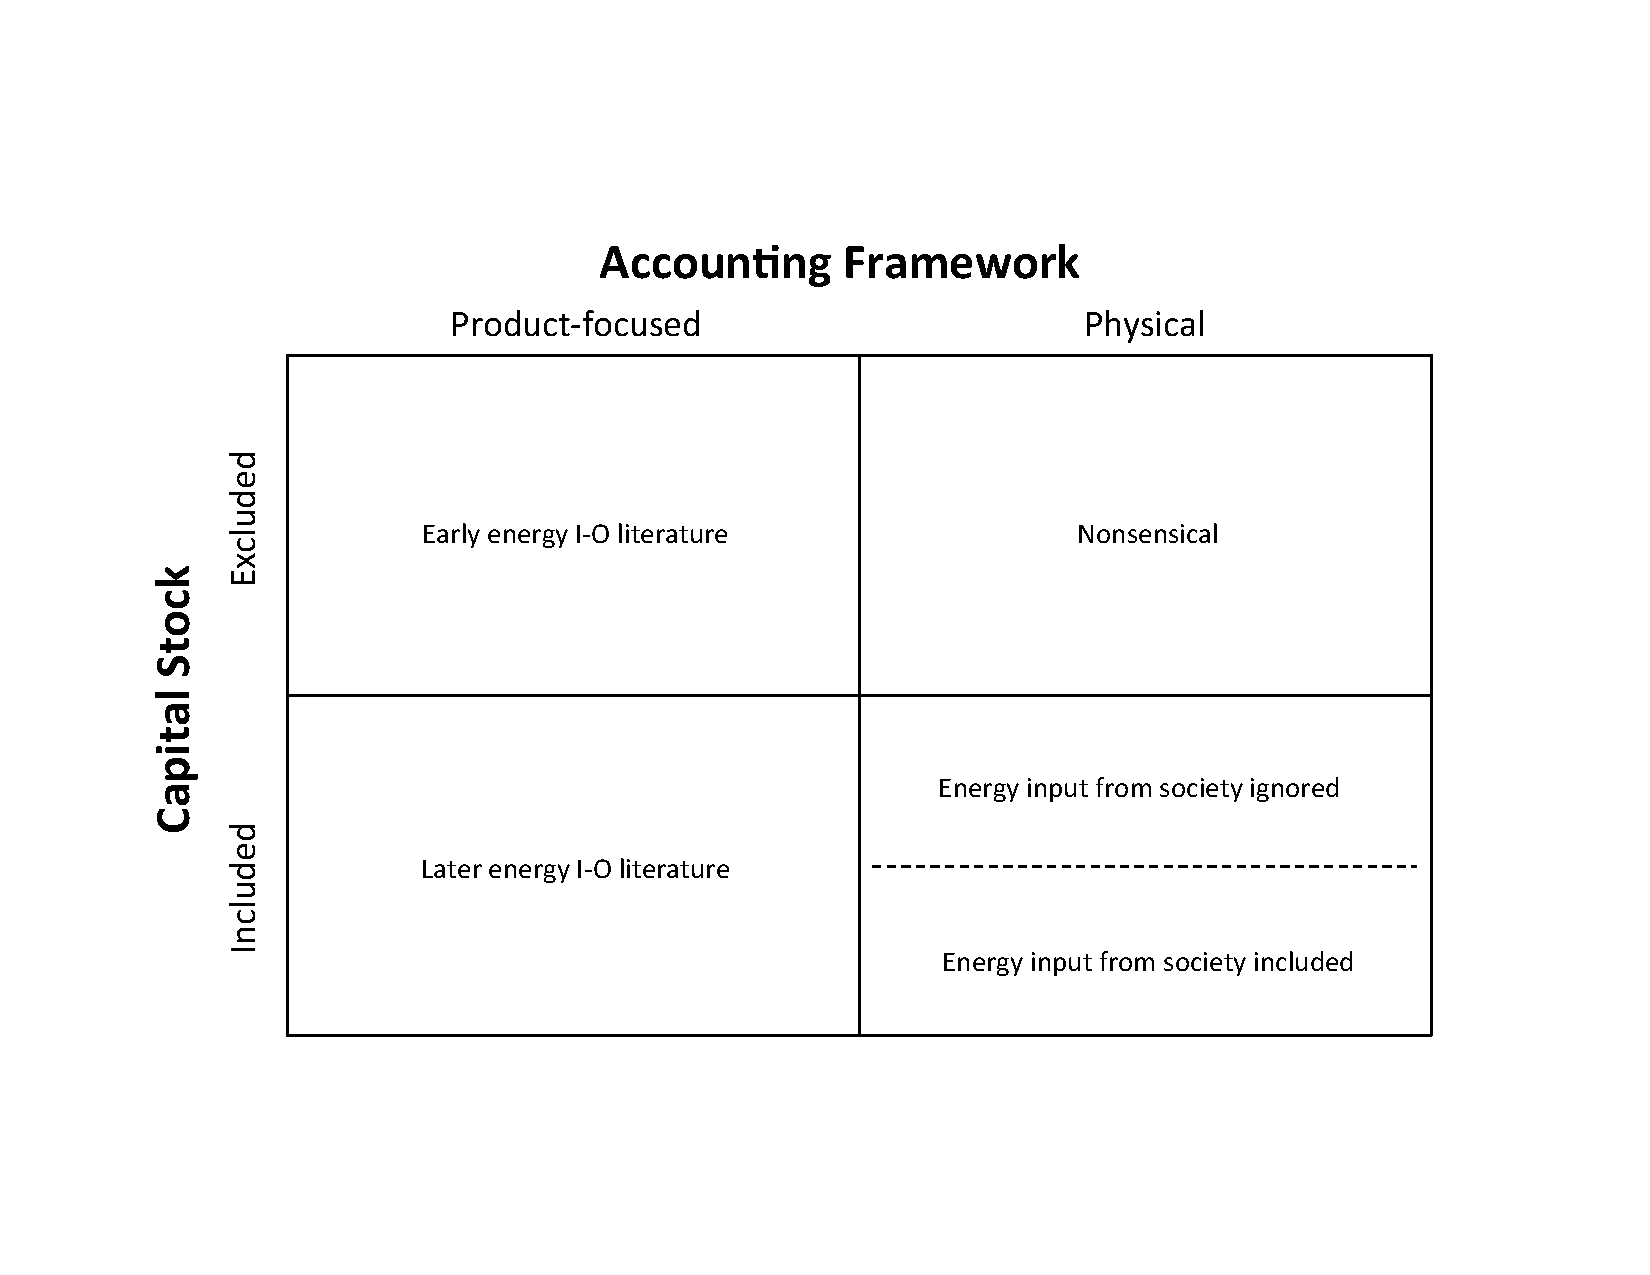
\includegraphics[width=0.8\linewidth]{Part_3/Chapter_Implications/Images/Grid.pdf}
	\caption[Coordinates of analysis for implications for the I-O method]{Coordinates of analysis for implications for the I-O method.}
	\label{fig:coords_of_analysis}
\end{figure}


%+++++++++ I-O implications: product-based vs. physical ++++++++++
\subsection{Product-based vs.\ physical approaches}
\label{sec:prod_vs_physical}
%+++++++++

The distinction between product-focused and physical
accounting system approaches is located in the columns
of Figure~\ref{fig:coords_of_analysis}.
A physical accounting system strictly follows materials 
through the economy. 
Embodied energy is accounted with the material stock or material flow
in which it resides.
For example, energy embodied within wastes ($\vec{B}_{waste}$) 
is not assigned to economic products. 
Rather, the energy embodied in wastes flows from sectors 
to the biosphere \emph{with the waste material}.
In contrast, a product-focused accounting system assigns 
energy embodied in wastes to the products of the sector.
Both product-based and physical accounting systems 
assign direct energy ($\dot{E}$) consumed by each sector
to the products of each sector.

Equation~\ref{eq:B_prod_physical_excluding_K} 
describes the outflow of embodied energy from sector $j$ 
exclusive of capital stock 
for a physical accounting system 
that neglects capital stock (upper-right quadrant of Figure~\ref{fig:coords_of_analysis}).\footnote{Equation~\ref{eq:B_prod_physical_excluding_K} 
is used for illustrative purposes only. 
We argue in Section~\ref{sec:capital_stock}
that a physical accounting system that neglects capital stock is nonsensical.}

\begin{equation} \label{eq:B_prod_physical_excluding_K}
	\dot{B}_{j}^{'}
	= \sum\limits_{i=1}^{n} \dot{B}_{ij}^{'} 
	- \dot{B}_{j,waste}
	+ \dot{Q}_{j0}
\end{equation}

\noindent{}Variables written with a ``prime''
(e.g.~$\dot{B}_{j}^{'}$) indicate definitions and terms that include only 
resource~($\dot{R}$) and short-lived~($\dot{S}$) flows 
and exclude capital flows~($\dot{K}$) and stock~($K$).
The term~$\dot{B}_{j,waste}$ represents the energy embodied 
within wasted resource~($\dot{R}_{j0}$) 
and short-lived~($\dot{S}_{j0}$) material flows.
The term is subtracted, because waste material flows are not assigned 
to the product~($\dot{B}_{j}^{'}$) in a physical accounting system.

In contrast, Equation~\ref{eq:B_prod_product_excluding_K} describes the outflow 
of embodied energy from sector~$j$
exclusive of capital stock ($\dot{B}_{j}^{'}$)
for a product-focused accounting system 
(upper left quadrant of Figure~\ref{fig:coords_of_analysis}).

\begin{equation} \label{eq:B_prod_product_excluding_K}
	\dot{B}_{j}^{'}
	= \sum\limits_{i=1}^{n} \dot{B}_{ij}^{'} 
	+ \dot{Q}_{j0}
\end{equation}

\noindent{}Notice that Equation~\ref{eq:B_prod_product_excluding_K} 
does not subract the energy embodied in waste resource and short-lived material
flows ($\dot{B}_{j,waste}$) on the right side, 
because product-focused accounting systems assign energy embodied in wastes
to products.


%+++++++++ I-O implications: Capital stock ++++++++++
\subsection{Capital stock}
\label{sec:capital_stock}
%+++++++++

The rows of Figure~\ref{fig:coords_of_analysis}
represent the role of capital stock in an accounting system.
During the earliest years of the I-O method applied to energy analysis 
(prior to the mid-1970s) capital stocks were ignored, 
both as flows or as stocks.
In essence, the state of the art was located in the upper-left quadrant
of Figure~\ref{fig:coords_of_analysis}.
In time, Kirkpatrick~\cite{Kirkpatrick:1974te}, 
Bullard and Herendeen~\cite{Bullard-III:1975aa},
and Casler~\cite{Casler:1983uy} attempted to 
include inflows of capital stock in a product-focused
accounting system, thereby moving the state of the art 
to the lower-left quadrant of Figure~\ref{fig:coords_of_analysis}.

In this manuscript, Equation~\ref{eq:epsilon_leontief_with_A} 
provides a means of estimating the energy intensity of economic sectors.

\begin{equation}
	\boldsymbol{\varepsilon} 
	= {(\vec{I} - \vec{A}^{\mathrm{T}})}^{-1}\hat{\vec{X}}^{-1}
		\left[\vec{E}_{0} 
				+ \vec{T}_{1} 
				- \frac{\mathrm{d}\vec{B}_{K}}{\mathrm{d}t} 
				- \vec{B}_{waste}
				- \hat{\boldsymbol{\gamma}}_{B}\vec{B}_{K}
		\right].\tag{\ref{eq:epsilon_leontief_with_A}}
\end{equation}

\noindent{}Thus, we take Equation~\ref{eq:epsilon_leontief_with_A} as the starting point
for discussion of the implications of our framework
for the I-O method.

To see the effect of the move from the upper-left to the lower-left
quadrant of Figure~\ref{fig:coords_of_analysis}, 
it is important to clearly understand both the assumptions and data that were used.
Energy analysts in the mid-1970s were utilizing the BEA I-O tables,
which do not include captial flows. 
Thus, this early literature implicitly assumes that 

\begin{equation} \label{eq:a_prime_lit}
	a_{ij}^{'} 
	\equiv \frac{\dot{X}_{ij,\dot{R}} + \dot{X}_{ij,\dot{S}}}
				{\dot{X}_{j,\dot{R}} + \dot{X}_{j,\dot{S}}}.
\end{equation}

\noindent{}Comparison between Equations~\ref{eq:aij_def_expanded}
and~\ref{eq:a_prime_lit}
highlights the fact that the early literature neglects flows of capital stock
($\dot{X}_{\dot{K}}$).
Thus, the the input-output matrix in the early literature
($\vec{A^{'}}$) is

\begin{equation} \label{eq:A_matrix_def_literature}
	\vec{A}^{'} 
	=
	\begin{bmatrix}
		a_{22}^{'} & a_{23}^{'}	\\
		a_{32}^{'} & a_{33}^{'}	
	\end{bmatrix}.
\end{equation}

\noindent{}Furthermore, the early literature implicitly defines 
energy intensity as

\begin{equation}
	\varepsilon_{j}^{'} 
	= \frac{\dot{T}_{j}^{'}}{\dot{X}_{j}^{'}},
\end{equation}

\noindent{}again, implicitly ignoring both the value and energy embodied within
flows of capital.

These implicit assumptions lead to the equation for energy intensity
found in most of the early literature

\begin{equation} \label{eq:intensity_upper_left}
	\boldsymbol{\varepsilon}^{'}
	= {\left( \vec{I} - {\vec{A}^{'}}^{\mathrm{T}} \right)}^{-1}
		{\left( \hat{\vec{X}}^{'}  \right)}^{-1}
		\vec{E}_{0}.
\end{equation}

\noindent{}In Figure~\ref{fig:coords_of_analysis}, 
Equation~\ref{eq:intensity_upper_left} would be located in the upper-left:
product-focused, excludes captial, neglects energy input from society.

Bullard and Herendeen~\cite{Bullard-III:1975aa}, 
following Kirkpatrick~\cite{Kirkpatrick:1974te}
added flows of capital stock as inputs to each sector~\cite[Figure~5]{Bullard-III:1975aa},
and, in so doing, changed Equation~\ref{eq:intensity_upper_left}
to Equation~\ref{eq:intensity_lower_left}.

\begin{equation} \label{eq:intensity_lower_left}
	\boldsymbol{\varepsilon}^{'}
	= {\left( \vec{I} - {\vec{A}^{'}}^{\mathrm{T}} \right)}^{-1}
		{\left( \hat{\vec{X}}^{'}  \right)}^{-1}
		\left[ \vec{E}_{0}
			  + \sum\limits_{i=1}^{n} \dot{B}_{ij} \right]
\end{equation}

\noindent{}We note that there was no attempt to redefine $\vec{A}^{'}$
or $\boldsymbol{\varepsilon}^{'}$.
Their approach to including capital stocks (within a product-focused
accounting system) assigned
all energy embodied captial stock to the products of the sector.
And, their product-focused accounting system
did not include an embodied energy stock 
for each economic sector ($\vec{B}$).
Thus, Equation~\ref{eq:intensity_lower_left} represents 
a partial step toward developing 
a method for estimating energy intensity ($\boldsymbol{\varepsilon}$)
that fully accounts for capital stock.

We agree with Kirkpatrick~\cite{Kirkpatrick:1974te}, 
Bullard and Herendeen~\cite{Bullard-III:1975aa},
and Casler~\cite{Casler:1983uy} that capital stock
is important and should be included in an accounting system.
But, we recommend that inclusion of capital stock should
be done within in a \emph{physical} accounting system, 
i.e.\ we should move from the lower-left to the lower-right
quadrant of Figure~\ref{fig:coords_of_analysis}.
Specifically, capital should be included 
(a) as a stock that can accumulate and (b) on all outflow streams,
not just on inflow streams.
Furthermore, capital should be included in the definition 
of the input-output table ($\vec{A}$) and 
energy intensity ($\boldsymbol{\varepsilon}$).

Our recommendation is based on the believe that
accounting for stocks of capital is essential for developing a coherent view
of the structure of an economy. 
Stocks of capital are essential to the production process:
without machines and factories, cars cannot be produced. 
Thus, the buildup of capital stock (and associated embodied energy) 
within economic sectors is an essential aspect of industrialization.
Carefully tracking (on a physical, as opposed to financial, basis) 
capital stock is essential for understanding the network effects of 
upstream energy demand as new industries and products arise 
(e.g., electric vehicles). 
Finally, maintenance of captial stock becomes an important 
driver of demand, especially in mature economies.

In a physical accounting system that includes capital stock
(such as the one we propose), 
energy embodied within accumulated capital stock
is not assigned to products ($\vec{P}$); 
rather, accumulated embodied energy is assigned to a stock of embodied energy
for each sector ($\vec{B}_{K}$).

A physical accounting system that fully includes capital stock
yields Equation~\ref{eq:intensity_lower_left}. 

\begin{equation} \label{eq:intensity_lower_right}
	\boldsymbol{\varepsilon}
	= {\left( \vec{I} - {\vec{A}}^{\mathrm{T}} \right)}^{-1}
		{\left( \hat{\vec{X}}  \right)}^{-1}
		\left[ \vec{E}_{0}
			  - \frac{\mathrm{d}\vec{B}_{K}}{\mathrm{d}t}
			  - \vec{B}_{waste} \right].
\end{equation}

\noindent{}Differences between Equation~\ref{eq:intensity_lower_right}
and Equation~\ref{eq:intensity_lower_left} include:

\begin{itemize}
	\item{$\boldsymbol{\varepsilon}$ appears rather than $\boldsymbol{\varepsilon}^{'}$,
	because both embodied energy and value of capital is included 
	in the definition of energy intensity,}
	\item{Equation~\ref{eq:intensity_lower_right} does not have
	the $\sum\limits_{i=1}^{n} \dot{B}_{ij}$ term, 
	because embodied energy flows are already included in $\vec{A}$,}
	\item{$\hat{\vec{X}}$ appears rather than $\hat{\vec{X}}^{'}$,
	because energy embodied in product streams is include in $\hat{\vec{X}}$,}
	\item{Equation~\ref{eq:intensity_lower_right} subtracts
	$\frac{\mathrm{d}\vec{B}_{K}}{\mathrm{d}t}$,
	because accumulation of energy embodied in the stock of capital ($K$)
	for a sector
	is not assigned to products of the sector, and}
	\item{Equation~\ref{eq:intensity_lower_right} subtracts $\vec{B}_{waste}$,
	because energy embodied in waste products is not assigned to 
	products of the sector.}
\end{itemize}

At this point, it is instructive to look back at the 
product-focused vs. physical discussion in Section~\ref{sec:prod_vs_physical}.
We understand the argument for a product-focused accounting system
that includes capital stock (lower-left quadrant of Figure~\ref{fig:coords_of_analysis}):
namely that capital stock and waste exist 
solely due to product demand, 
therefore energy embodied in capital and waste should be assigned to products. 
However, the product-focused system that includes capital stock (lower-left quadrant of
Figure~\ref{fig:coords_of_analysis})
masks structural aspects of economies
that we believe are essential to fully understanding how energy flows 
through economies, namely the accumulation of capital within sectors.
The metabolic metaphor provides guidance here.  
If we create a model of an organism that neglects 
tissues that accumulate embodied energy,
the organism has nothing with which to 
absorb, process, waste, or otherwise exchange
material with the biosphere.
The organism doesn't physically exist (in the model)!
Neglecting to account for the stock of capital (and its embodied energy) 
is tantamount to assuming that economic production occurs out of nothing!





In 1969, Eugene Odum outlined a number of 
defining characteristics of both \emph{developmental},
i.e.\ growing,
and \emph{mature} ecosystems in terms of key
properties of the system.~\cite{Odum1969}
The main message was that ecosystems cannot
grow indefinitely in their (photosynthetic)~production~($P$)
due mainly to the necessity of increasing maintenance
demands as the amount of (biomass) capital
stock~($B$) increases.
Eventually, all production is used in this manner
and growth ceases 
$\left(\frac{\mathrm{d}P}{\mathrm{d}t} = 0\right)$.

In the early stages of ecosystem development,
the ratio $\frac{P}{B}$,
i.e.\ the energy production per unit of biomass stock,
 is high.
 As the ecosystem approaches maturity,
 this ratio decreases.
 Put another way,
 the inverse ratio $\frac{B}{P}$,
 i.e.\ the biomass stock (maintained) per unit of energy produced,
 starts low and asymptotically increases to a maximum
 when growth (in both $P$ and $B$) has ceased. 
The ratio $\frac{B}{P}$ may be high or low\footnote{The
 value of $\frac{B}{P}$ at maturity (and the time taken to reach it)
 ``may vary not only with different climatic 
 and physiographic situations but also with
 different ecosystem attributes in the same physical 
 environment.''\cite[p.263]{Odum1969}}
and may therefore be considered a measure of 
 the ``efficiency'' to which the ecosystem applies
 energy production toward
 the goal of maintaining biomass stock.
 
 Turning back to economies,
 Daly has,
 in our view,
 correctly applied this concept to societal patterns
 of consumption.~\cite{Daly1995}
 Our framework,
 analogously suggests that,
 as capital stock~$\left(\vec{B}_{K}\right)$ increases,
 an increasing flow of energy production~$\left(\vec{E}_{0}\right)$
 will be needed to maintain that stock.
 Our economies (and economic models) are still locked
 on the goal of growth.
 We have outlined a possible reason for the difficulty
 of maintaining high levels of economic growth
 as an economy matures.
 Eventually,
 we believe,
 our economies must learn to maximize the $\frac{B}{P}$
 ratios of our economies 
 $\left(\frac{\vec{B}_{K}}{\vec{E}_{0}}\right)$
 **** MCD---should this be 
 $\left(\frac{\mathrm{d}\vec{B}_{K}}{\mathrm{d}\vec{E}_{0}}\right)$
 ****

%+++++++++ I-O implications: Energy input from society ++++++++++
\subsection{Energy input from society}
\label{sec:energy_from_society}
%+++++++++












%%%%%%%%%% I-O implications: estimating epsilon %%%%%%%%%%
\subsection{Estimating $\boldsymbol{\varepsilon}$}
\label{sec:estimating_epsilon-implications_chapter}
%%%%%%%%%%


In this manuscript, Equation~\ref{eq:epsilon_leontief_with_A} 
provides a means of estimating the energy intensity of economic sectors:

\begin{equation}
	\boldsymbol{\varepsilon} 
	= {(\vec{I} - \vec{A}^{\mathrm{T}})}^{-1}\hat{\vec{X}}^{-1}
		\left[\vec{E}_{0} 
				+ \vec{T}_{1} 
				- \frac{\mathrm{d}\vec{B}_{K}}{\mathrm{d}t} 
				- \vec{B}_{waste}
				- \hat{\boldsymbol{\gamma}}_{B}\vec{B}_{K}
		\right].\tag{\ref{eq:epsilon_leontief_with_A}}
\end{equation}

\noindent{}The I-O literature~\cite{Bullard1975,Casler1984}, 
uses a similar, but different, equation. 
In this section, we unpack the (often unstated) assumptions in the literature
and develop an expression that translates
between our analysis and the analysis typically found in the literature. 

We begin by noting that 
flows of capital stock ($\dot{K}$) are not included in the 
standard I-O tables from the
Bureau of Economic Analysis (BEA).\footnote{See
Section~\ref{sec:Data} for a discussion of data needs.}
Historically, only a few energy analysts attempted to include the effect
of capital flows on energy intensity ($\boldsymbol{\varepsilon}$). 
Bullard~\cite{Bullard1975} added capital stock purchases as an input
to each economic sector.
Casler~\cite{Casler:1983uy} attempted to correct the BEA's
input-output tables prior to applying the I-O method.
However, the present analysis (based on 
the model of material, energy, and value flows presented 
in Chapters~\ref{chap:materials}--\ref{chap:value})
affords the opportunity
to develop a mathematically-rigorous analysis
of the effects of physical depreciation.

Given that the BEA I-O tables do not include captial flows, 
much of the literature implicitly assumes that 

% \begin{equation} \label{eq:a_prime_lit}
% 	a_{ij}^{'} 
% 	\equiv \frac{\dot{X}_{ij,\dot{R}} + \dot{X}_{ij,\dot{S}}}
% 				{\dot{X}_{j,\dot{R}} + \dot{X}_{j,\dot{S}}}.
% \end{equation}
% 
% \noindent{}Variables written with a ``prime''
% (e.g.\ $a^{'}$) indicate definitions and terms as used in the literature.
% Comparison between Equations~\ref{eq:aij_def_expanded}
% and~\ref{eq:a_prime_lit}
% indicates that the literature neglects capital stock flows 
% ($\dot{X}_{\dot{K}}$).
% Thus, the the input-output matrix in the literature
% ($\vec{A^{'}}$) is
% 
% \begin{equation} \label{eq:A_matrix_def_literature}
% 	\vec{A}^{'} 
% 	=
% 	\begin{bmatrix}
% 		a_{22}^{'} & a_{23}^{'}	\\
% 		a_{32}^{'} & a_{33}^{'}	
% 	\end{bmatrix}.
% \end{equation}
% 
Furthermore, the literature assumes that production does not include
capital stock (again, due to the fact that the BEA does not include 
capital flows in the standard I-O tables) such that

\begin{equation}
	\hat{\vec{X}}^{'} = \hat{\vec{X}}_{\dot{R}} + \hat{\vec{X}}_{\dot{S}},
\end{equation}

\noindent{}whereas our formulation (Equation~\ref{eq:X_hat_matrix_def})
includes capital flows explicitly:

\begin{equation}
	\hat{\vec{X}} = \hat{\vec{X}}_{\dot{R}} + \hat{\vec{X}}_{\dot{S}} + \hat{\vec{X}}_{\dot{K}}.
\end{equation}

The literature writes Equation~\ref{eq:epsilon_leontief_with_A} as

\begin{equation} \label{eq:epsilon_leontief_with_A_literature}
	\boldsymbol{\varepsilon^{'}} 
	= {\left( \vec{I} - {\vec{A}^{'}}^{\mathrm{T}} \right)}^{-1}
	% {    \hat{  \vec{X}  }  }  ^{-1}
	{\left( \hat{\vec{X}}^{'} \right)}^{-1}
	\vec{E}_{0}.
\end{equation}

The differences between Equations~\ref{eq:epsilon_leontief_with_A}
and~\ref{eq:epsilon_leontief_with_A_literature} are clear. 
Most of the literature neglects
\begin{itemize}
	\item{capital flows (by using $\vec{A}^{'}$ and $\hat{\vec{X}}^{'}$
			instead of $\vec{A}$ and $\hat{\vec{X}}$),}
	\item{energy input from society ($\vec{T}_{1}$),}
	\item{accumulation of embodied energy in the economy 
			$\left( \frac{\mathrm{d}\vec{B}_{K}}{\mathrm{d}t} \right)$,}
	\item{the embodied energy of scrap resource	and short-lived material flows 
			($\dot{\vec{B}}_{waste}$) and}
	\item{depreciation $\hat{\boldsymbol{\gamma}}_{B} \vec{B}_{K}$}
\end{itemize}

\noindent{}when estimating the energy intensity  
of economic sectors ($\boldsymbol{\varepsilon}^{'}$).
In other words, most energy analysts using the input-output method
have, to date, and perhaps unwittingly, assumed 
a developed-world ($\vec{T}_{1} \ll \vec{E}_{0}$),
steady state economy\index{steady-state economy}
$\left( \frac{\mathrm{d}\mathrm{\vec{B}}_{K}}{\mathrm{d}t}  
= \vec{0} \right)$ 
with 
no capital flow (using $\vec{A}^{'}$ and $\hat{\vec{X}}^{'}$),
no waste ($\vec{B}_{waste} = \vec{0}$), and
no depreciation ($\hat{\boldsymbol{\gamma}}_{B} = \vec{0}$).

Equations~\ref{eq:epsilon_leontief_with_A} 
and~\ref{eq:epsilon_leontief_with_A_literature}
have one common term, $\vec{E}_{0}$.
We can solve Equation~\ref{eq:epsilon_leontief_with_A_literature}
for $\vec{E}_{0}$ 

\begin{equation}
	\vec{E}_{0}
	= \hat{\vec{X}}^{'} \left( \vec{I} - {\vec{A}^{'}}^\mathrm{T} \right) \boldsymbol{\varepsilon^{'}} 
\end{equation}

\noindent{}and substitute into
Equation~\ref{eq:epsilon_leontief_with_A}
to obtain an expression that relates $\boldsymbol{\varepsilon}$ 
and $\boldsymbol{\varepsilon}^{'}$

\begin{align}
	\boldsymbol{\varepsilon}
	=& {\left( \vec{I} - \vec{A}^{\mathrm{T}} \right)}^{-1} \hat{\vec{X}}^{-1}
			\hat{\vec{X}}^{'} \left( \vec{I} - {\vec{A}^{'}}^{\mathrm{T}} \right) 
			\boldsymbol{\varepsilon^{'}} 
	& + {\left( \vec{I} - \vec{A}^{\mathrm{T}} \right)}^{-1} \hat{\vec{X}}^{\mathrm{-1}}
	\left[ \vec{T}_{1} - \frac{\mathrm{d}\vec{B}_{K}}{\mathrm{d}t}  
			- \vec{B}_{waste} - \hat{\boldsymbol{\gamma}}_{B} \vec{B}_{K} \right].
\end{align}

**** Next, substitute a dB/dt equation with $\alpha$ into the equation. ****

**** Possibly include $\alpha$ below. 
Tie the $\alpha$ term to how Bullard and Herendeen 
simply added capital stock to embodied energy inputs to the sector. ****

The following subsections discuss these assumptions.

**** Ensure that each assumption is covered below. ****



%+++++++++ Negligible energy input from society ++++++++++
\subsubsection{Ignoring capital flows}
%+++++++++



%+++++++++ Negligible energy input from society ++++++++++
\subsubsection{Negligible energy input from society $\left( \vec{T}_{1} = \vec{0} \right)$}
%+++++++++

Energy input from society to the economy ($\vec{T}_{1}$)
is ``muscle work'' supplied by working humans 
and draught animals.\cite{Ayres:2003ec,Ayres:2010ug,Warr:2012cg} 
This muscle work term ($\vec{T}_{1}$) should include
all upstream energy required to make the labor available.\footnote{It is important
to note that $\vec{T}_{1}$ should include all upstream energy,
because at this point in the development of this framework 
for accounting materials, energy, and value,
we are assuming that Final Consumption (Sector 1) is exogenous to the economy 
(Sectors 2 and 3), 
and upstream energy consumption needs to be included manually.
However, in Section~\ref{sec:what_is_endogenous}, we show that Final Consumption
can be endogenized.
Once endogenized, the energy intensity of Final Consumption ($\varepsilon_{1}$) 
will automatically include the upstream energy required to make labor available.
(See Appendix~\ref{chap:infinite_series}.)

It is important to note, too, that labor can have very high energy intensity, 
because $\varepsilon_{1}$ includes the energy required to supply food and transport
to workers.} 
For industrialized economies, muscle work 
is likely to provide only a small fraction
of the energy input from fossil fuels ($\vec{E}_{0}$),
so neglecting $\vec{T}_{1}$ causes negligible error when
estimating energy intensity ($\boldsymbol{\varepsilon}$) by
Equation~\ref{eq:epsilon_leontief_with_A_literature}.
However, for some agrarian\index{economy!agrarian} 
and developing economies\index{economy!developing}, 
in which $\vec{T}_{1}$ and $\vec{E}_{0}$ 
could be on the same order of magnitude,
neglecting $\vec{T}_{1}$ could cause errors
in estimates of $\boldsymbol{\varepsilon}$.
To the extent that $\vec{T}_{1}$ 
is significant relative to $\vec{E}_{0}$,
Equation~\ref{eq:epsilon_leontief_with_A_literature}
will underpredict the energy intensity of the economy.

Accurate estimation of the energy intensity of economic output ($\boldsymbol{\varepsilon}$)
requires independent knowledge of the rate at which society supplies
energy to the economy~($\vec{T}_{1}$). 
Ayres and Warr have estimated human and animal muscle work
input to the economy for a few developed countries.\cite{Ayres:2010ug}
We recommend that more of this work be done 
in the future for many more countries.


%+++++++++ Negligible accumulation of embodied energy ++++++++++
\subsubsection{Negligible accumulation of embodied energy
$\left( \left. \frac{\mathrm{d}\vec{B}_{K}}{\mathrm{d}t} \right|_{\mathrm{other}} = \vec{0} \right)$}
%+++++++++

As discussed in detail below (Section~\ref{sec:implications_for_development}),
the accumulation of embodied energy 
$\left( \left. \frac{\mathrm{d}\vec{B}_{K}}{\mathrm{d}t} \right|_{\mathrm{other}} \right)$
in society and the economy
can be considered a marker of economic ``development.''

% **** 
% Mik says: Daly talks about this in terms 
% of Odum's B/P vs P/B ratios for growing vs.\ steady systems.
% ****

Equation~\ref{eq:epsilon_leontief_depreciation_simplification} 
shows that embodied energy accumulation within economic sectors 
exclusive of depreciation
$\left( \left. \frac{\mathrm{d}\vec{B}_{K}}{\mathrm{d}t} \right|_{\mathrm{other}} \right)$ 
decreases the energy intensity of products~($\boldsymbol{\varepsilon}$),
because incoming energy becomes embodied within capital stock rather than products.
Costanza points out that traditional
``input-output methodology does not include capital stocks explicitly, 
since a static equillibrium is assumed.''\cite{Costanza:1980ww}
Comparison with Equation~\ref{eq:epsilon_leontief_with_A_literature}
shows that the method in the literature will overestimate the energy intensity
of economic products ($\boldsymbol{\varepsilon}$) when 
$\left. \frac{\mathrm{d}\vec{B}_{K}}{\mathrm{d}t} \right|_{\mathrm{other}} > 0$.

Rapidly growing economies (as measured by GDP), such as China and India today,
are expected to have rather large positive values in the  
$\left. \frac{\mathrm{d}\vec{B}_{K}}{\mathrm{d}t} \right|_{\mathrm{other}}$ vector,
while slowly-growing, industrialized economies, 
such as the United States and the United Kingdom,
are expected to have rather smaller values in the 
$\left. \frac{\mathrm{d}\vec{B}_{K}}{\mathrm{d}t} \right|_{\mathrm{other}}$ vector.
Applying Equation~\ref{eq:epsilon_leontief_with_A_literature} 
(i.e., assuming a steady-state economy\index{economy!steady-state})
will tend to overestimate the energy intensity 
of economic products for rapidly growing economies such as China and India.
The approximate magnitude of mis-estimation remains unknown, because
estimates of the magnitude of
$\left. \frac{\mathrm{d}\vec{B}_{K}}{\mathrm{d}t} \right|_{\mathrm{other}}$
have yet to be made.

Equation~\ref{eq:epsilon_leontief_depreciation_simplification} shows that 
accurate estimation of the energy intensity of economic output ($\boldsymbol{\varepsilon}$)
requires \emph{independent} knowledge of the rate 
at which embodied energy accumulates in the capital stock of the economy 
$\left( \left. \frac{\mathrm{d}\vec{B}_{K}}{\mathrm{d}t} \right|_{\mathrm{other}} \right)$,
and all estimates of energy intensity ($\boldsymbol{\varepsilon}$) to date have assumed 
$\left. \frac{\mathrm{d}\vec{B}_{K}}{\mathrm{d}t} \right|_{\mathrm{other}} = 0$.\footnote{To 
our knowledge, there are no independent estimates 
of the accumulation rate of embodied energy in the economy
$\left( \left. \frac{\mathrm{d}\vec{B}_{K}}{\mathrm{d}t} \right|_{\mathrm{other}} \right)$.}
Furthermore, Equation~\ref{eq:epsilon_leontief_depreciation_simplification} 
cannot be used to estimate the accumulation rate of energy embodied in 
capital stock by solving for 
$\left( \left. \frac{\mathrm{d}\vec{B}_{K}}{\mathrm{d}t} \right|_{\mathrm{other}} \right)$,
because that approach would require independent knowledge
of the energy intensity of economic sectors ($\boldsymbol{\varepsilon}$).
Alternatively, Equation~\ref{eq:C_embodied_energy_accounting_123_with_depreciation} 
could be simplified using the 
methods of Section~\ref{sec:intensity_capital_correction} to obtain

\begin{equation} \label{eq:C_embodied_energy_accounting_123_with_depreciation_simplified}
	\left. \frac{\mathrm{d}B_{K_{j}}}{\mathrm{d}t} \right|_{\mathrm{other}}
	= \sum\limits_{i=1}^n\dot{B}_{ij} 
	- \dot{B}_{j}
	- \dot{B}_{waste,j0}
	+ \dot{Q}_{j0},
\end{equation}

\noindent{}but this approach would require independent knowledge of the 
embodied energy of all inter-sectoral material transfers in the entire economy.

At present, the situation appears to be a catch-22. 
However, a way around the problem may come from application
of bottom-up, process-based methods to the problem 
of estimating the accumulation of embodied energy 
in economic sectors. 
Some steps have been made in this direction.\cite{brandt2013calculating}
But, clearly, further work focused on estimating the relative magnitudes of 
$\left. \frac{\mathrm{d}\vec{B}_{K}}{\mathrm{d}t} \right|_{\mathrm{other}}$,
$\vec{T}_{1}$, and $\vec{B}_{waste}$ 
will benefit energy analysts who utilize the I-O method.


%+++++++++ Negligible embodied energy in waste ++++++++++
\subsubsection{Negligible energy embodied in waste ($\vec{B}_{waste} = 0$)}
%+++++++++

If the energy embodied in waste resources ($\dot{R}$)
and short-lived materials ($\dot{S}$) are ignored,
Equation~\ref{eq:epsilon_leontief_depreciation_simplification}
shows that estimates of the energy intensity of economic products 
($\boldsymbol{\varepsilon}$) will be too high.
We are unaware of any estimates of the energy embodied in wasted
material in an economy.  
But, one might develop a metric for the resource material effiency of an 
economic sector ($\eta_{\dot{R}}$)\nomenclature[h]{$\eta_{\dot{R}}$}{resource efficiency [kg/kg]} 
such that

\begin{equation} \label{eq:manufacturing_effiency}
	\eta_{\dot{R},j}
	\equiv \frac{\dot{P}_{j}}{\sum\limits_{i=1}^{n} \dot{R}_{ij}}.
\end{equation}

\noindent{}With the above definition, 
the scrap rate for resources could be expressed as
$(1~-~\eta_{\dot{R}}) \sum\limits_{i=1}^{n} \dot{R}_{ij}$.
Allwood et.\ al.~\cite[p. 193]{allwood2012sustainable} 
used a process-based approach to manufacturing efficiencies
for metals used in manufacturing. 
The data are summarized in Table~\ref{tab:scrap_rates}.

\begin{table}
\caption{Manufacturing efficiencies (Equation~\ref{eq:manufacturing_effiency}) 
for selected manufactured goods.\cite{allwood2012sustainable}}
\begin{center}
\begin{tabular} {r @{\hspace{2em}} l}
	\toprule
	Product & Manufacturing Efficiency [\%] \\
	\midrule
	Steel I-beam             & 90 \\
	Car Door Panel           & 50 \\
	Aluminium Drink Can      & 50 \\
	Aircraft Wing Skin Panel & 10 \\
	\bottomrule
\end{tabular}
\end{center}
\label{tab:scrap_rates}
\end{table}

Furthermore, one could assume that the rate
of short-lived materials ($\dot{S}$) used by a sector could be given as a 
fraction of the resource ($\dot{R}$) use rate such that:

\begin{equation}
	\rho_{\dot{S},j}
	\equiv \frac{\dot{S}_{j0}}{\sum\limits_{i=1}^{n} \dot{R}_{ij}}
	= \frac{\sum\limits_{i=1}^{n} \dot{S}_{ij}}{\sum\limits_{i=1}^{n} \dot{R}_{ij}}.
\end{equation} \nomenclature[r]{$\rho_{\dot{S}}$}{ratio of short-lived material
flow to resource inputs [kg/kg]}

With the above definitions, the waste resource rate from an economic sector
can be given as

\begin{equation}
	\dot{R}_{j0} + \dot{S}_{j0}
	= (1 - \eta_{\dot{R}_{j}} + \rho_{\dot{S},j}) \sum\limits_{i=1}^{n} \dot{R}_{ij}.
\end{equation}

\noindent{}The embodied energy in the waste materials would need to be estimated
from the embodied energy of the incoming resource and short-lived material flows.

However, it could be argued that the embodied energy content 
of waste from the production process should be 
assigned to the products of a sector.\footnote{This approach 
is similar to assigning waste heat energy from an
economic sector to the embodied energy of its products.
See Section~\ref{subsec:A_first_law_embodied} and
Equation~\ref{eq:A_dB1/dt} for a discussion of this approach.}
If so, Equation~\ref{eq:epsilon_leontief_depreciation_simplification}
could be modified as

\begin{equation} \label{eq:epsilon_leontief_without_waste}
	\boldsymbol{\varepsilon} 
	= {(\vec{I} - \vec{A}^{\mathrm{T}})}^{-1}\hat{\vec{X}}^{-1}
		\left[\vec{E}_{0} 
				+ \vec{T}_{1} 
				- \left. \frac{\mathrm{d}\vec{B}_{K}}{\mathrm{d}t} \right|_{\mathrm{other}}
		\right],
\end{equation}

\noindent{}and the waste rates are unneeded.

Further work focused on estimating values for 
$\eta_{\dot{R}}$ and $\rho_{\dot{S}}$
and the the energy embodied in waste flows 
will benefit energy analysts who utilize the I-O method.

A second set of implications for the I-O method 
comes from one of the ways that 
the energy intensity vector ($\boldsymbol{\varepsilon}$)
is often used: to estimate energy demand from the biosphere ($\vec{E}_{0}$).


%%%%%%%%%% I-O implications: estimating E %%%%%%%%%%
\subsection{Estimating $\vec{E}_{0}$}
%%%%%%%%%%

The assumptions of Equation~\ref{eq:epsilon_leontief_with_A_literature}
may cause another challenge for energy analysts. 
As shown in 
Equation~\ref{eq:epsilon_leontief_depreciation_simplification}
and discussed in Section~\ref{sec:estimating_epsilon-implications_chapter} above, 
the I-O method can be used to estimate energy intensities 
for each sector of the economy ($\boldsymbol{\varepsilon}$). 
With $\boldsymbol{\varepsilon}$ values in hand,
and assuming that $\boldsymbol{\varepsilon}$ is constant with respect to time,
energy analysts have estimated changes in energy demand 
from the biosphere ($\vec{E}_{0}$) 
as the output of economic sectors ($\hat{\vec{X}}$) 
increases or decreases by solving 
Equation~\ref{eq:epsilon_leontief_with_A_literature} 
for $\vec{E}_{0}$:

\begin{equation} \label{eq:Leontief_lit_solved_for_E}
	\vec{E}_{0} 
	= \hat{\vec{X}}(\vec{I} - \vec{A}^{\mathrm{T}})\boldsymbol{\varepsilon}.
\end{equation}

When Equation~\ref{eq:epsilon_leontief_with_A_literature}
is modified to account for accumulation of embodied energy 
in the economy 
$\left( \left. \frac{\mathrm{d}\vec{B}_{K}}{\mathrm{d}t} \right|_{\mathrm{other}} \right)$,
waste materials ($\vec{B}_{waste}$), and
energy supplied by society to the economy ($\vec{T}_{1}$),
we see that energy demands ($\vec{E}_{0}$) must be calculated differently. 
Solving Equation~\ref{eq:epsilon_leontief_depreciation_simplification} 
for $\vec{E}_{0}$ gives 

\begin{equation} \label{eq:Leontief_solved_for_E_with_embodied_depreciation}
	\vec{E}_{0} 
	= \hat{\vec{X}}
		(\vec{I} - \vec{A}^{\mathrm{T}})
		\boldsymbol{\varepsilon} 
	+ \left. \frac{\mathrm{d}\vec{B}_{K}}{\mathrm{d}t} \right|_{\mathrm{other}}
	+ \vec{B}_{waste}
	- \vec{T}_{1}.
\end{equation}

\noindent{}Comparison of Equations~\ref{eq:Leontief_lit_solved_for_E} 
and~\ref{eq:Leontief_solved_for_E_with_embodied_depreciation}
shows that to the extent that embodied energy accumulation,
exclusive of physical depreciation
$\left( \left. \frac{\mathrm{d}\vec{B}_{K}}{\mathrm{d}t} \right|_{\mathrm{other}} \right)$
is non-zero, estimates of energy demand ($\vec{E}_{0}$) using 
Equation~\ref{eq:Leontief_lit_solved_for_E} are too low. 
If wastes ($\vec{B}_{waste}$) are ignored, 
estimates of energy demand ($\vec{E}_{0}$) using 
Equation~\ref{eq:Leontief_lit_solved_for_E} will be too low. 
And, if energy input from society to the economy ($\vec{T}_{1}$) is significant,
estimates of energy demand ($\vec{E}_{0}$) using 
Equation~\ref{eq:Leontief_lit_solved_for_E} will be too high. 

At this time, the relative magnitudes of $\vec{E}_{0}$,
$\left. \frac{\mathrm{d}\vec{B}_{K}}{\mathrm{d}t} \right|_{\mathrm{other}}$,
$\vec{B}_{waste}$, and $\vec{T}_{1}$ are unknown. 
Further work to clarify these magnitudes will be beneficial
for energy analysts who employ the I-O method.
 

%%%%%%%%%% Implications %%%%%%%%%%
\section{Implications for economic ``development''}
\label{sec:implications_for_development}
%%%%%%%%%%

**** Becky, write a paragraph here about alternative measures of development. 
Discuss Daly's Genuine Progress Indicator (which includes natural capital, Mik to verify)
and Gross National Happiness and other. ****

Economic ``development''\footnote{We choose to use the word ``development'' to
describe expanding economies, despite significant misgivings about the term. 
The unambiguously positive connotations of the words ``development'' and ``developed''
fail to capture the nuances of travel along economic development paths:
there are so many ways in which life experience in ``developed'' countries 
is both better and worse than life in ``developing'' countries.
We hope to convey our misgivings by surrounding these words with quotation marks in this text.}
is usually ``measured''
by Gross Domestic Product\index{Gross Domestic Product} (GDP).
With reference to Figure~\ref{fig:C_value}, $GDP$ is calculated by

\begin{equation} \label{eq:GDP_def}
	GDP
	= \sum\limits_{j=2}^{n} \dot{X}_{j}
\end{equation}

\noindent{}where $n$ is the number of sectors in the economy.
Equation~\ref{eq:GDP_def} clearly shows that 
$GDP$ is a \emph{flow} of value in units of \$/year.

As a given economy moves along its ``development'' path,
sectors within the economy accumulate capital stock 
($K$, typically expressed in units of dollars)
and associated embodied energy 
($B_{K}$, expressed in units of joules).
If we turn this around, 
accumulation of embodied energy in economic sectors and society 
could be considered a \emph{proxy} for ``development.''\footnote{Embodied energy 
as a proxy for development may be overly focused on capital stock, 
therefore one-dimensional, and reductive, 
but GDP and other measures are open to similar criticism.}
Equation~\ref{eq:Dev_Integral_Economy} indicates how accumulated
embodied energy in the capital stock 
of an economy ($\vec{B}_{K}$) could be calculated:

\begin{equation} \label{eq:Dev_Integral_Economy}
	\vec{B}_{K}(t) 
	= \vec{B}_{K}(0) 
	+ \int_{t=0}^{t=t} \frac{\mathrm{d}\vec{B}_{K}}{\mathrm{d}t}\mathrm{d}t,
\end{equation}

\noindent{}where $\vec{B}_{K}$ is given by Equation~\ref{eq:B_vec_def}.
Equation~\ref{eq:Dev_Integral_Economy} clearly shows
that energy embodied energy in capital stock ($\vec{B}_{K}$) 
is a \emph{stock} (in units of joules), not a flow.

The behavior of $\vec{B}_{K}$ with respect to
$\left. \frac{\mathrm{d}\vec{B}_{K}}{\mathrm{d}t} \right|_{\mathrm{other}}$ 
is vitally important. 
As an economy transitions from agrarian to industrialized, 
its capital stock ($K$) and associated embodied energy ($B_{K}$)
grows ever larger. 
The outflow of depreciated capital stock and its associated embodied energy 
will occur at a faster rate, too.
As increasingly large amounts of energy are embodied 
in the capital stock of an economy ($B_{K}$), 
Equation~\ref{eq:matrix_leontief} shows that
increasingly large energy extraction rates ($\vec{E}_{0}$) 
are required to maintain capital stock 
in the sectors of the economy
to offset the effects of depreciation 
($\hat{\boldsymbol{\gamma}}_{K} \vec{B}_{K}$),
assuming that $\frac{\mathrm{d}\vec{B}_{K}}{\mathrm{d}t} \ge 0$ 
is desired. 

During a period of rapid industrialization and infrastructure build-out, 
we expect both $GDP$ and energy embodied in the economy ($\vec{B}_{K}$)
to increase.
But, there is no guarantee that $GDP$ and $\vec{B}_{K}$ move 
in the same direction at all times.
Industrialized economies may experience $GDP$ growth while 
the stock of embodied energy in the economy ($\vec{B}_{K}$) remains nearly constant,
because the economy is running circles to overcome the effects of depreciation.
There can be a time lag between movements of GDP and $\vec{B}_{K}$, too.
At the beginning of an economic downturn (defined as prolonged GDP reduction),
capital stock and associated embodied energy ($\vec{B}_{K}$) will remain approximately constant:
GDP moves but $\vec{B}_{K}$ doesn't.
But as the GDP decline continues, 
maintenance flows for capital stock will be reduced
and depreciation will overtake maintenance leading to a decline in $\vec{B}_{K}$. 
If economic decline is associated with significant external 
infrastructure investment (such as occurred in post-colonial Africa),
GDP may decrease 
while the stock of energy embodied in the economy ($\vec{B}_{K}$) increases 
due to foreign aid focused on infrastructure enhancement.
**** We may want a better example here.
Does foreign aid inflows count toward GDP\@?
Did this actually occur for any country in post-colonial Africa? 
--MKH ****

A second possible measure of economic ``development'' is another \emph{stock}, 
wealth:

\begin{equation} \label{eq:Dev_Integral_Wealth}
	X_{j}(t) 
	= X_{j}(0) 
	+ \int_{t=0}^{t=t} \frac{\mathrm{d}X_{j}}{\mathrm{d}t}\mathrm{d}t,
\end{equation}

\noindent{}where $j=1$ for societal wealth 
and $j \in [2,n]$ for corporate wealth, both measured in dollars.
In fact, capital (as represented by energy embodied in infrastructure, $\vec{B}_{K}$) and 
financial resources (as represeted by $X_{2 \ldots n}$) 
are complimentary factors of production for economic processes. 
But, we can go further than linking capital with financial resources.
If capital~($\vec{B}_{K}$) is to be useful, we need financial resources
or currency~($\dot{X}$) to 
\begin{itemize}
	\item{purchase direct energy~($\dot{E}$) to power the capital,
	\item{purchase resources~($\dot{R}$) to feed the capital, and}
	\item{pay workers~(represented 
	by societal energy input to the economy,~$\vec{T}_{1}$) 
	to operate the capital.}
} 
\end{itemize}

Thus, economic growth could be considered a ``fully coupled'' problem:
understanding it requires breadth of knowledge and appreciation for 
interactions among many important factors.
Each of the factors discussed above 
($\dot{X}$, $\vec{B}_{K}$, $\dot{E}$, $\dot{R}$, and $\vec{T}_{1}$)
is necessary, but not sufficient, for economic growth.

Our framework serves highlight to several issues in economic ``growth.'' 
Should it be measured by a stock or a flow? 
Which measure is most appropriate? 
What roles do currency, capital stock, energy, resources, and labor
play in economic processes?
These are overlapping and complementary areas of inquiry.
We encourage further research in all of these areas.


%%%%%%%%%% Implications %%%%%%%%%%
\section{Implications for recycling, reuse, and dematerialization}
\label{sec:recycling}
%%%%%%%%%%

%**** Mik: take a shot a rewriting. **** MCD---shot taken! ****

Dematerialization is the idea that economic activity can be unlinked 
from material or energy demands.\cite{FischerKowalski:2011uo} 
One method for dematerializing an economy 
is reuse and recycling of materials from both
short-lived goods
$\left(\vec{B}_{waste}\right)$
and depreciation of 
capital 
stock~$\left(\hat{\boldsymbol{\gamma}}_{K}\vec{B}_{K}\right)$
that would otherwise have
been expended to the biosphere.\footnote{Another 
method  of dematerialization is 
substitution away from production of material goods 
and toward information and services
in an economy.}
%**** MCD - I removed the following sentence as I don't agree with it. ****
% The impact of recycling can be seen in the I-O formulation 
% only when depreciation and accumulation terms are included. 

In Chapter~\ref{chap:intensity},
we defined the rate of accumulation 
of embodied energy within the economy
$\left(\frac{\mathrm{d}\vec{B}_{K}}{\mathrm{d}t}\right)$
by the following equation:

\begin{equation}
	\frac{\mathrm{d}\vec{B}_{K}}{\mathrm{d}t} 
	= \vec{E}_{0}
	+ \vec{T}_{1}
	+ \hat{\vec{X}} (\vec{A}^{\mathrm{T}} - \vec{I})\boldsymbol{\varepsilon} 
	- \vec{B}_{waste}
	- \hat{\boldsymbol{\gamma}}_{K}\vec{B}_{K}\tag{\ref{eq:matrix_leontief}}
\end{equation}

One effect of recycling is to reduce the magnitude 
of the waste 
$\left(\vec{B}_{waste}\right)$
and depreciation 
$\left(\hat{\boldsymbol{\gamma}}_{K}\right)$ 
terms,
since for a given level of capital 
stock~$\left(\vec{B}_{K}\right)$
the amount of depreciation to the 
biosphere $\left(\hat{\boldsymbol{\gamma}}_{K}\vec{B}_{K}\right)$
will be lower due to the fraction that
is now recycled.
As can be seen by looking at 
Equation~\ref{eq:matrix_leontief},
this indicates that 
recycling of material in an economy, 
by reducing both $\vec{B}_{waste}$ 
and~$\hat{\boldsymbol{\gamma}}_{K}$, 
puts \emph{upward} pressure on the accumulation of 
energy embodied in capital stock
$\left(\frac{\mathrm{d}\vec{B}_{K}}{\mathrm{d}t}\right)$.

Recycling has a mixed effect on energy demand ($\vec{E}_{0}$). 
Because recycled materials can displace newly-produced material 
in the economy and society, 
recycling will tend to reduce energy demand ($\vec{E}_{0}$). 
However, recycling processes require energy to operate, 
thereby putting upward pressure on energy demand ($\vec{E}_{0}$). 
If the energetic cost of recycling is lower than that of obtaining materials
from virgin resources, as is the case for many metals, 
e.g.\ aluminum~\cite{Chapman1975}, 
the result is a net reduction of energy demand 
from the biosphere ($\vec{E}_{0}$). 
Berry and Fels found that recycling of the material in automobiles
would result in 12,640 kW-hr of energy reduction per vehicle.\cite[p. 15]{Berry:1973vo}
Therefore recycling will also put \emph{downward} pressure on 
the growth of embodied energy in the economy
$\left(\frac{\mathrm{d}\vec{B}_{K}}{\mathrm{d}t}\right)$. 

If recycling produces a net reduction in energy demand ($\vec{E}_{0}$), 
% i.e.\ if the effect of displaced production dominates over the effect 
% of energy consumed in recycling processes, 
the upward pressure on growth 
$\left(\frac{\mathrm{d}\vec{B}_{K}}{\mathrm{d}t}\right)$ 
from decrease in depreciation 
$\left(\hat{\boldsymbol{\gamma}}_{K}\right)$ 
and the downward pressure on growth 
from net reduction in energy demand 
$\left(\vec{E}_{0}\right)$ 
can offset each other.
Under those conditions, 
the accumulation rate of energy embodied in capital stock
$\left(\frac{\mathrm{d}\vec{B}_{K}}{\mathrm{d}t}\right)$ 
will remain near zero 
and total embodied energy 
$(\vec{B}_{K})$ will remain constant. 
In that scenario, 
dematerialization can occur: 
reduced material and energy input ($\vec{E}_{0}$) 
can be accompanied by 
no change in
the growth of the economy
$\left(\frac{\mathrm{d}\vec{B}_{K}}{\mathrm{d}t}\right)$.
However,
as will be discussed in Section~\ref{sec:material_quality},
recycled materials can never entirely replace
the need for new materials.

%%%%%%%%%% Implications %%%%%%%%%%
\section{Comparison to a steady-state economy}
\label{sec:SSE}
%%%%%%%%%%

As discussed in Chapter~\ref{chap:intro},
the human economy is a subset of the biosphere which is a
finite, non-growing system,
\emph{open} to flows of solar energy but \emph{closed}
to material transfers.
Because the biosphere is finite in size,
the human economy cannot physically grow indefinitely.
The concept of a non-growing or ``steady-state'' economy
has existed for centuries.
There are a number of different
conditions that may characterize a system as steady-state.
In thermodynamics,
the condition of a zero rate of accumulation
of some stock, $x$
$\left(\frac{\mathrm{d}x}{\mathrm{d}t} = 0\right)$
is normally used to define steady state conditions.\footnote{Or,
more generally,
a change in any property over time
$\left(\frac{\partial p}{\partial t}\right)$.}
Other conditions that might define a steady-state
economy are:
a constant rate of material through-put,
constant GDP, or constant population.
Our framework,
as outlined here,
can address the first three steady-state conditions.
The fourth condition, constant population, could be
accommodated with some adaptation of the 
framework. 
The issue of human population as part of society's
capital stock is addressed in Section~\ref{sec:people_as_stock}.


%+++++++++++++++++++++++++++++++++++++++++++
%+++++++++ Constant capital stock ++++++++++
%+++++++++++++++++++++++++++++++++++++++++++
\subsection{Constant level of capital stock}

In Chapter~\ref{chap:materials}, 
we introduced Equation~\ref{eq:C_CV_all_b}:

\begin{align}\tag{\ref{eq:C_CV_all_b}}
	- \frac{\mathrm{d}R_{0}}{\mathrm{d}t}										&
	=\sum_{j}\frac{\mathrm{d}K_{j}}{\mathrm{d}t}
	+ \sum_{i,j}\dot{S}_{ij}
	+ \sum_{j}\gamma_{K_{j}}K_{j}.
\end{align}

\noindent{}which indicates that 
the depletion of natural resources in the 
biosphere~$\left(- \frac{\mathrm{d}R_{0}}{\mathrm{d}t}\right)$
by the economy
is used for the purposes of:

\begin{itemize}
	\item{increasing man-made capital stocks
	within the economy~$\left(\frac{\mathrm{d}K_{j}}{\mathrm{d}t}\right)$,}
	\item{providing short-lived goods exchanged within the
	economy~$\left(\dot{S}_{ij}\right)$, and}
	\item{overcoming depreciation of man-made
	capital stocks~$\left(\sum_{j}\gamma_{K_{j}}K_{j}\right)$.}
\end{itemize}

Assuming,
first,
that a steady-state economy exists when the level
of capital stock remains constant
$\left(\sum_{j}\frac{\mathrm{d}K_{j}}{\mathrm{d}t}=0\right)$,\footnote{Note
that the steady-state condition does not preclude expansion
of some sectors of the economy, provided that there is 
equal contraction elsewhere.}
we can see that Equation~\ref{eq:C_CV_all_b}
reduces to:

\begin{align}\label{eq:C_CV_all_c}
	- \frac{\mathrm{d}R_{0}}{\mathrm{d}t}										&
	= \sum_{i,j}\dot{S}_{ij}
	+ \sum_{j}\gamma_{K_{j}}K_{j}.
\end{align}

A number of interesting concepts may be understood in
relation to Equation~\ref{eq:C_CV_all_c}. 
Firstly,
if our steady-state economy is to be supported
sustainably,
then withdrawal of natural resources from the biosphere
$\left(\frac{\mathrm{d}R_{0}}{\mathrm{d}t}\right)$
had better be at some rate lower than the biosphere
can replenish the natural capital stocks. 
In reality, 
$\frac{\mathrm{d}R_{0}}{\mathrm{d}t}$
is really the sum of many different resources
(flora and fauna, water) each of which will have
its own natural rate of regeneration.
As such, 
the sustainability criterion  is a vector of values,
one for each natural resource.

Secondly,
the steady state condition 
$\left(\sum_{j}\frac{\mathrm{d}K_{j}}{\mathrm{d}t}=0\right)$
says nothing about the transfer rates of short-lived goods 
within in the economy $\left(\sum_{i,j}\dot{S}_{ij}\right)$
or the depreciation of capital stock back to the biopshere
$\left(\sum_{j}\gamma_{K_{j}}K_{j}\right)$.
Equation~\ref{eq:C_CV_all_c} indicates that 
the higher the rates of these flows,
the greater the rate of depletion of
natural resources, and the more difficult it will be to
meet the sustainability condition 
(that the withdrawal rate of natural resources from the biosphere
is lower than the biosphere
replenishment rate).
Within industrial society,
the flow of short-lived goods 
(packaging,
paper products,
disposable tableware,
cutlery,
and napkins)
is large,
and, presumably, attaining a sustainable steady-state economy
will be difficult.
This definition of steady state 
$\left(\sum_{j}\frac{\mathrm{d}K_{j}}{\mathrm{d}t}=0\right)$
does not necessarily coincide with sustainability.

As discussed in Chapter~\ref{chap:materials},
the rate of depreciation ($\gamma_{K}$) is inversely
proportional to the average lifetime of capital stock---as
the average lifetime of capital stock decreases,
the rate of depreciation of capital stock increases which
increases the draw on natural resources (by Equation~\ref{eq:C_CV_all_c}).
It is likely that the average lifetime of capital stock has
decreased over the last century, 
due to a decrease in durability of capital stock
(the average table built today is not as durable as the average table
built in the early twentieth century)
and also due to increasing proportions of consumer electronics
with short lifetimes (cell phones, laptops, tablets).
Decreasing lifetime causes higher rates of flow for
replacement materials.
In the absence of extreme recycling of materials,
these large replacement flows place large demands on
natural resources.

Thirdly,
the maintenance flows necessary to overcome
depreciation
$\left(\sum_{j}\gamma_{K_{j}}K_{j}\right)$
are proportional to the magnitude of the capital
stock ($K_{j}$).
As such,
a larger stock of capital requires
greater draw on natural resources and is thus harder
to maintain within any sustainability constraint.
These points emphasize that constant capital stock
(or analogously constant population)
is not a sufficient condition for environmental sustainability.


%++++++++++++++++++++++++++++++++++++++++
%+++++++++ Constant throughput ++++++++++
%++++++++++++++++++++++++++++++++++++++++
\subsection{Constant material throughput}

Herman Daly has placed great emphasis on a steady-state
economy as having a constant rate of material throughput 
\cite{Daly1977, Daly1997}
which, as discussed above, should be below biophysical limits
if sustainability is to be achieved.
This is often referred to as the ``scale'' issue---how 
large is the (currently growing) human economy in relation
to the finite, non-growing biosphere of which it is a sub-system?
Growth of the human economy must either displace other natural
ecosystems (replacing old growth forest for crops)
or deplete natural capital stocks, be they 
renewable (fisheries) or 
non-renewable (fossil fuels).
As shown in Figure~\ref{fig:C_materials},
material throughput is composed of two distinct processes:
exchange of material \emph{from} the biosphere 
\emph{into} the economy (extraction)
and exchange of material \emph{from} the economy
\emph{into} biosphere (waste and depreciation).
We may characterizing constant material throughput
as either constant rate of extraction, constant rate of
waste disposal, or both.
In the language of our framework, we could write:

\begin{align}\label{eq:const_throughput}
	\frac{\mathrm{d}}{\mathrm{d}t}\left(\dot{R}_{0}\right)		&
	= 0																							\\
	\frac{\mathrm{d}}{\mathrm{d}t}\left(\dot{S}_{0}\right)		&
	= 0																						\\
	\sum\limits_{i}
			\left[
				\frac{\mathrm{d}}{\mathrm{d}t}\left(\dot{R}_{i0}\right)
				+ \frac{\mathrm{d}}{\mathrm{d}t}\left(\dot{S}_{i0}\right)
				+ \frac{\mathrm{d}}{\mathrm{d}t}\left(\dot{K}_{i0}\right)
			\right]																			&
	= 0.
\end{align}

The above equations say nothing about the level 
of man-made capital stock ($K$)
or the flow rate of short-lived goods ($\dot{S}$).
Thus, within the constant throughput constraint,
increasingly effective use of materials could
theoretically allow increasing accumulation
of man-made capital ($K$) 
and increasing flow of short-lived goods ($\dot{S}$)
as society learns to use resources better.
Eventually,
physical limits would entail that capital
stock could no longer be increased.
Presumably,
society would desire that the throughput of
materials would be within levels that could
be sustained by the biosphere,
both at the input side---natural 
resources extracted at rates lower
than natural regeneration rates---and 
at the output side---wastes emitted 
at rates below which
the biosphere can assimilate.


%++++++++++++++++++++++++++++++++++++++++
%+++++++++ Constant GDP ++++++++++
%++++++++++++++++++++++++++++++++++++++++
\subsection{Constant GDP}

The issue of GDP and economic ``development'' 
has already been discussed in 
Section~\ref{sec:implications_for_development}. 
However,
the case of zero growth in GDP was not.
Within our framework,
a condition of constant GDP would be
characterized by the following equation:

\begin{equation}\label{eq:const_GDP}
	\frac{\mathrm{d}}{\mathrm{d}t}\left(GDP\right)
	=	\sum\limits_{j}\frac{\mathrm{d}}{\mathrm{d}t}\left(\dot{X}_{j}\right)
	= 0
\end{equation}

Since,
under the subjective theory of value,
no value is attributed to the flow of materials
to or from the biosphere,
it is unclear what the impact constant GDP would be
on capital stock ($K$)
or material throughput
(extraction and waste disposal).
If we constrained $\dot{R}_{0}$ and
$\dot{S}_{0}$, 
it is likely that economic growth would 
decrease or even become zero or negative
$\left(\frac{\mathrm{d}}{\mathrm{d}t}\left(GDP\right) \leq 0\right)$.
It is conceivable that constraining
economic growth may act to constrain
material throughput,
though this is certainly not assured.
Many authors argue that increasing GDP
no longer guarantees increasing welfare~\cite{G-R1975a, Wackernagel1996,
Cobb1999, Daly2006, Costanza2014} 
for two main reasons:
\begin{itemize}
	\item firstly, that the costs of growth in GDP, 
	some of which are added as benefits into GDP 
	but also externalities (especially environmental) 
	which are not counted at all, outweigh any benefit 
	that comes from increasing GDP;\@ and
	\item secondly, that increasing GDP serves to
	increase relative income inequality,
	despite increasing absolute income,
	which decreases welfare for both rich and poor 
	alike.~\cite{Daly2006}
\end{itemize}

Furthermore,
the argument for increasing GDP as a means
to alleviate poverty is undermined by this second point.
The world's poor are poor because they cannot afford to
buy food and other goods due to their \emph{relative} poverty,
not because there is an \emph{absolute} lack of these goods.
The rising tide raises all boats,
but the (growing) luxury cruisers soon capsize 
the (shrinking) dinghies.



**** MCD---Becky, can you speak to this? 
This last paragraph is way outside my area of expertise and
is a little bit ``soap boxy''. ****

**** Discuss maintenance vs.\ accumulation flows? 
Is this a better place to discuss this issue? Can refer to
Section 6.5 and Odum B/P vs. P/B. ****

%****** Mik: Finish this section. 
%In terms of what a SSE would look like in the I-O framework, 
%at first blush, I would think that dB/dt = 0 is one aspect.  
%Also, with no growth, inflow rates = depreciation rates.  
%The larger that B is for any society, the larger E must be (to overcome depreciation).  
%To minimize E, hyper-recycling is probably useful.  
%Those are at least a place to start. ******
%
%****** In our discussion, 
%we also addressed the attempts at SSE from point of view of society. 
%In order to achieve this goal \emph{without} recycling, 
%the goods and services sector should have to increase extraction to offset decreasing ore grade, 
%the energy sector should have to increase extraction of energy 
%to allow increasing extraction (unless efficiency could make up the gap: unlikely) 
%in which case the SSE would be violated from these two and from the POV of the earth.
%******


\bibliographystyle{unsrt}
\bibliography{../../EROI_review_v2}


% Always give a unique label
% and use \ref{<label>} for cross-references
% and \cite{<label>} for bibliographic references
% use \sectionmark{}
% to alter or adjust the section heading in the running head
%% Instead of simply listing headings of different levels we recommend to let every heading be followed by at least a short passage of text. Furtheron please use the \LaTeX\ automatism for all your cross-references and citations.

%% Please note that the first line of text that follows a heading is not indented, whereas the first lines of all subsequent paragraphs are.

%% Use the standard \verb|equation| environment to typeset your equations, e.g.
%
%% \begin{equation}
%% a \times b = c\;,
%% \end{equation}
%
%% however, for multiline equations we recommend to use the \verb|eqnarray|
%% environment\footnote{In physics texts please activate the class option \texttt{vecphys} to depict your vectors in \textbf{\itshape boldface-italic} type - as is customary for a wide range of physical subjects.}.
%% \begin{eqnarray}
%% a \times b = c \nonumber\\
%% \vec{a} \cdot \vec{b}=\vec{c}
%% \label{eq:01}
%% \end{eqnarray}

%% \subsection{Subsection Heading}
%% \label{subsec:2}
%% Instead of simply listing headings of different levels we recommend to let every heading be followed by at least a short passage of text. Furtheron please use the \LaTeX\ automatism for all your cross-references\index{cross-references} and citations\index{citations} as has already been described in Sect.~\ref{sec:2}.

%% \begin{quotation}
%% Please do not use quotation marks when quoting texts! Simply use the \verb|quotation| environment -- it will automatically render Springer's preferred layout.
%% \end{quotation}


%% \subsubsection{Subsubsection Heading}
%% Instead of simply listing headings of different levels we recommend to let every heading be followed by at least a short passage of text. Furtheron please use the \LaTeX\ automatism for all your cross-references and citations as has already been described in Sect.~\ref{subsec:2}, see also Fig.~\ref{fig:1}\footnote{If you copy text passages, figures, or tables from other works, you must obtain \textit{permission} from the copyright holder (usually the original publisher). Please enclose the signed permission with the manucript. The sources\index{permission to print} must be acknowledged either in the captions, as footnotes or in a separate section of the book.}

%% Please note that the first line of text that follows a heading is not indented, whereas the first lines of all subsequent paragraphs are.

% For figures use
%
%% \begin{figure}[b]
%% \sidecaption
% Use the relevant command for your figure-insertion program
% to insert the figure file.
% For example, with the option graphics use
%% \includegraphics[scale=.65]{figure}
%
% If not, use
%\picplace{5cm}{2cm} % Give the correct figure height and width in cm
%
%% \caption{If the width of the figure is less than 7.8 cm use the \texttt{sidecapion} command to flush the caption on the left side of the page. If the figure is positioned at the top of the page, align the sidecaption with the top of the figure -- to achieve this you simply need to use the optional argument \texttt{[t]} with the \texttt{sidecaption} command}
%% \label{fig:1}       % Give a unique label
%% \end{figure}


%% \paragraph{Paragraph Heading} %
%% Instead of simply listing headings of different levels we recommend to let every heading be followed by at least a short passage of text. Furtheron please use the \LaTeX\ automatism for all your cross-references and citations as has already been described in Sect.~\ref{sec:2}.

%% Please note that the first line of text that follows a heading is not indented, whereas the first lines of all subsequent paragraphs are.

%% For typesetting numbered lists we recommend to use the \verb|enumerate| environment -- it will automatically render Springer's preferred layout.

%% \begin{enumerate}
%% \item{Livelihood and survival mobility are oftentimes coutcomes of uneven socioeconomic development.}
%% \begin{enumerate}
%% \item{Livelihood and survival mobility are oftentimes coutcomes of uneven socioeconomic development.}
%% \item{Livelihood and survival mobility are oftentimes coutcomes of uneven socioeconomic development.}
%% \end{enumerate}
%% \item{Livelihood and survival mobility are oftentimes coutcomes of uneven socioeconomic development.}
%% \end{enumerate}


%% \subparagraph{Subparagraph Heading} In order to avoid simply listing headings of different levels we recommend to let every heading be followed by at least a short passage of text. Use the \LaTeX\ automatism for all your cross-references and citations as has already been described in Sect.~\ref{sec:2}, see also Fig.~\ref{fig:2}.

%% Please note that the first line of text that follows a heading is not indented, whereas the first lines of all subsequent paragraphs are.

%% For unnumbered list we recommend to use the \verb|itemize| environment -- it will automatically render Springer's preferred layout.

%% \begin{itemize}
%% \item{Livelihood and survival mobility are oftentimes coutcomes of uneven socioeconomic development, cf. Table~\ref{tab:1}.}
%% \begin{itemize}
%% \item{Livelihood and survival mobility are oftentimes coutcomes of uneven socioeconomic development.}
%% \item{Livelihood and survival mobility are oftentimes coutcomes of uneven socioeconomic development.}
%% \end{itemize}
%% \item{Livelihood and survival mobility are oftentimes coutcomes of uneven socioeconomic development.}
%% \end{itemize}

%% \begin{figure}[t]
%% \sidecaption[t]
% Use the relevant command for your figure-insertion program
% to insert the figure file.
% For example, with the option graphics use
%% \includegraphics[scale=.65]{figure}
%
% If not, use
%\picplace{5cm}{2cm} % Give the correct figure height and width in cm
%
%% \caption{Please write your figure caption here}
%% \label{fig:2}       % Give a unique label
%% \end{figure}

%% \runinhead{Run-in Heading Boldface Version} Use the \LaTeX\ automatism for all your cross-references and citations as has already been described in Sect.~\ref{sec:2}.

%% \subruninhead{Run-in Heading Italic Version} Use the \LaTeX\ automatism for all your cross-refer\-ences and citations as has already been described in Sect.~\ref{sec:2}\index{paragraph}.
% Use the \index{} command to code your index words
%
% For tables use
%
%% \begin{table}
%% \caption{Please write your table caption here}
%% \label{tab:1}       % Give a unique label
%
% For LaTeX tables use
%
%% \begin{tabular}{p{2cm}p{2.4cm}p{2cm}p{4.9cm}}
%% \hline\noalign{\smallskip}
%% Classes & Subclass & Length & Action Mechanism  \\
%% \noalign{\smallskip}\svhline\noalign{\smallskip}
%% Translation & mRNA$^a$  & 22 (19--25) & Translation repression, mRNA cleavage\\
%% Translation & mRNA cleavage & 21 & mRNA cleavage\\
%% Translation & mRNA  & 21--22 & mRNA cleavage\\
%%Translation & mRNA  & 24--26 & Histone and DNA Modification\\
%%\noalign{\smallskip}\hline\noalign{\smallskip}
%%\end{tabular}
%%$^a$ Table foot note (with superscript)
%%\end{table}
%
%% \section{Section Heading}
%%\label{sec:3}
% Always give a unique label
% and use \ref{<label>} for cross-references
% and \cite{<label>} for bibliographic references
% use \sectionmark{}
% to alter or adjust the section heading in the running head
%% Instead of simply listing headings of different levels we recommend to let every heading be followed by at least a short passage of text. Furtheron please use the \LaTeX\ automatism for all your cross-references and citations as has already been described in Sect.~\ref{sec:2}.

%% Please note that the first line of text that follows a heading is not indented, whereas the first lines of all subsequent paragraphs are.

%%If you want to list definitions or the like we recommend to use the Springer-enhanced \verb|description| environment -- it will automatically render Springer's preferred layout.

%%\begin{description}[Type 1]
%%\item[Type 1]{That addresses central themes pertainng to migration, health, and disease. In Sect.~\ref{sec:1}, Wilson discusses the role of human migration in infectious disease distributions and patterns.}
%%\item[Type 2]{That addresses central themes pertainng to migration, health, and disease. In Sect.~\ref{subsec:2}, Wilson discusses the role of human migration in infectious disease distributions and patterns.}
%%\end{description}

%%\subsection{Subsection Heading} %
%% In order to avoid simply listing headings of different levels we recommend to let every heading be followed by at least a short passage of text. Use the \LaTeX\ automatism for all your cross-references and citations citations as has already been described in Sect.~\ref{sec:2}.

%% Please note that the first line of text that follows a heading is not indented, whereas the first lines of all subsequent paragraphs are.

%% \begin{svgraybox}
%% If you want to emphasize complete paragraphs of texts we recommend to use the newly defined Springer class option \verb|graybox| and the newly defined environment \verb|svgraybox|. This will produce a 15 percent screened box 'behind' your text.

%% If you want to emphasize complete paragraphs of texts we recommend to use the newly defined Springer class option and environment \verb|svgraybox|. This will produce a 15 percent screened box 'behind' your text.
%% \end{svgraybox}


%% \subsubsection{Subsubsection Heading}
%%Instead of simply listing headings of different levels we recommend to let every heading be followed by at least a short passage of text. Furtheron please use the \LaTeX\ automatism for all your cross-references and citations as has already been described in Sect.~\ref{sec:2}.

%% Please note that the first line of text that follows a heading is not indented, whereas the first lines of all subsequent paragraphs are.

%% \begin{theorem}
%% Theorem text goes here.
%% \end{theorem}
%
% or
%
%% \begin{definition}
%% Definition text goes here.
%% \end{definition}

%% \begin{proof}
%\smartqed
%% Proof text goes here.
%% \qed
%% \end{proof}

%%\paragraph{Paragraph Heading} %
%% Instead of simply listing headings of different levels we recommend to let every heading be followed by at least a short passage of text. Furtheron please use the \LaTeX\ automatism for all your cross-references and citations as has already been described in Sect.~\ref{sec:2}.

%% Note that the first line of text that follows a heading is not indented, whereas the first lines of all subsequent paragraphs are.
%
% For built-in environments use
%
%%\begin{theorem}
%%Theorem text goes here.
%%\end{theorem}
%
%%\begin{definition}
%%Definition text goes here.
%%\end{definition}
%
%%\begin{proof}
%%\smartqed
%% Proof text goes here.
%%\qed
%%\end{proof}
%
%% \begin{acknowledgement}
%% If you want to include acknowledgments of assistance and the like at the end of an individual chapter please use the \verb|acknowledgement| environment -- it will automatically render Springer's preferred layout.
%% \end{acknowledgement}
%
%% \section*{Appendix}
%% \addcontentsline{toc}{section}{Appendix}
%
%% When placed at the end of a chapter or contribution (as opposed to at the end of the book), the numbering of tables, figures, and equations in the appendix section continues on from that in the main text. Hence please \textit{do not} use the \verb|appendix| command when writing an appendix at the end of your chapter or contribution. If there is only one the appendix is designated ``Appendix'', or ``Appendix 1'', or ``Appendix 2'', etc. if there is more than one.

%% \begin{equation}
%% a \times b = c
%% \end{equation}
% Problems or Exercises should be sorted chapterwise
%% \section*{Problems}
%% \addcontentsline{toc}{section}{Problems}
%
% Use the following environment.
% Don't forget to label each problem;
% the label is needed for the solutions' environment
%% \begin{prob}
%% \label{prob1}
%% A given problem or Excercise is described here. The
%% problem is described here. The problem is described here.
%% \end{prob}

%% \begin{prob}
%% \label{prob2}
%% \textbf{Problem Heading}\\
%% (a) The first part of the problem is described here.\\
%% (b) The second part of the problem is described here.
%% \end{prob}


